\documentclass[rgb]{beamer}

\usepackage[english]{babel}
\usepackage[utf8]{inputenc}
\usepackage{xcolor}
\usepackage{listings}
\usepackage{adjustbox}
\usepackage{amsmath}
\usepackage{multirow}
\usepackage[linewidth=1pt]{mdframed}

% Graphics
\usepackage{graphicx}

\usepackage{tikz}
\usetikzlibrary{calc,shapes.multipart,chains,arrows}

% Font
\usepackage{paratype}
\setbeamerfont{frametitle}{family=\bf}

% Beamer theme settings
\usecolortheme{seagull}
\setbeamertemplate{itemize item}{\raisebox{0.8mm}{\rule{1.8mm}{1.2mm}}}
\usenavigationsymbolstemplate{} % no navigation buttons

\usepackage{listings}

% Define Language
\lstdefinelanguage{fsharp}
{
  % list of keywords
  morekeywords={
    and,
    do,
    else,
    exception,
    for,
    fun,
    function,
    if,
    in,
    let,
    match,
    module,
    mutable,
    open,
    of,
    rec,
    then,
    try,
    type,
    unsafe,
    use,
    val,
    when,
    while,
    with,
  },
  sensitive=true, % keywords are not case-sensitive
  morecomment=[l]{//}, % l is for line comment
%  otherkeywords={>,<,=,<=,>=,!,*,/,-,+,|,&,||,&&,==,=>},
  morestring=[b]" % defines that strings are enclosed in double quotes
}

% Define Colors
\usepackage{color}
\definecolor{eclipseBlue}{RGB}{42,0.0,255}
\definecolor{eclipseGreen}{RGB}{63,127,95}
\definecolor{eclipsePurple}{RGB}{127,0,85}

\newcommand{\fop}[1]{\mbox{\ttfamily\color{eclipseBlue}#1}}
\newcommand{\fw}[1]{\mbox{\ttfamily\bfseries\color{eclipsePurple}#1}}

% Set Language
\lstset{
  language={fsharp},
  basicstyle=\ttfamily, % Global Code Style
  captionpos=b, % Position of the Caption (t for top, b for bottom)
  extendedchars=true, % Allows 256 instead of 128 ASCII characters
  tabsize=2, % number of spaces indented when discovering a tab
  columns=fixed, % make all characters equal width
  keepspaces=true, % does not ignore spaces to fit width, convert tabs to spaces
  showstringspaces=false, % lets spaces in strings appear as real spaces
  breaklines=true, % wrap lines if they don't fit
  frame=trbl, % draw a frame at the top, right, left and bottom of the listing
  frameround=tttt, % make the frame round at all four corners
  framesep=4pt, % quarter circle size of the round corners
  numbers=left, % show line numbers at the left
  numberstyle=\small\ttfamily, % style of the line numbers
  commentstyle=\slshape\bfseries\color{eclipseGreen}, % style of comments
  keywordstyle=\bfseries\color{eclipsePurple}, % style of keywords
  stringstyle=\color{eclipseBlue}, % style of strings
  emph=[1] {
    false,
    true,
    Set,
    Map,
    List,
    ImgUtil,
    Pegs,
    String,
    Array,
    Array2D
  },
  emphstyle=[1]{\color{eclipseBlue}},
  moredelim=**[is][\color{red}]{@@}{@@}
}

\newcommand{\theyear}{2020}
\newcommand{\sem}[1]{[\![#1]\!]}
\newcommand{\seme}[1]{\sem{#1}\varepsilon}
\newcommand{\semzero}[1]{\sem{#1}_0}

\newcommand{\emptymap}{\{\}}
\newcommand{\fracc}[2]{\begin{eqnarray} \frac{\begin{array}{c} #1
    \end{array}}{\begin{array}{c} #2 \end{array}} \end{eqnarray}}
\newcommand{\sembox}[1]{\hfill \normalfont \mbox{\fbox{\(#1\)}}}
\newcommand{\sempart}[2]{\subsubsection*{\rm\em #1 \sembox{#2}}}
\newcommand{\axiom}[1]{\begin{eqnarray} \begin{array}{c} #1 \end{array} \end{eqnarray}}
\newcommand{\fraccn}[2]{\refstepcounter{equation}\mbox{$\frac{\begin{array}{c} #1 \end{array}}{\begin{array}{c} #2 \end{array}}$}~(\arabic{equation})}
\newcommand{\fraccc}[2]{\mbox{$\frac{\begin{array}{c} #1 \end{array}}{\begin{array}{c} #2 \end{array}}$}}
\newcommand{\onepart}[1]{\noindent\hfill#1\hfill~\vspace{2mm}}
\newcommand{\twopart}[2]{\noindent\hfill#1\hfill#2\hfill~\vspace{2mm}}
\newcommand{\threepart}[3]{\noindent\hfill#1\hfill#2\hfill#3\hfill~\vspace{2mm}}
%\newcommand{\axiomm}[1]{\refstepcounter{equation}\mbox{$\begin{array}{c} #1 \end{array}$}~(\arabic{equation})}
\newcommand{\axiomm}[1]{$\begin{array}{c} #1 \end{array}$}
%\newcommand{\ar}[1]{\stackrel{#1}{\longrightarrow}}
\newcommand{\vd}{\vdash}
\newcommand{\Ran}{{\rm Ran}}
\newcommand{\Dom}{{\rm Dom}}
\newcommand{\kw}[1]{\texttt{#1}}
\newcommand{\id}[1]{\mbox{\it{#1}}}
\newcommand{\rarr}{\rightarrow}
\newcommand{\eval}{\rarr}
\newcommand{\evals}{\leadsto}
\newcommand{\larr}{\leftarrow}

\newcommand{\head}[1]{\vspace{3mm} \textbf{\normalsize #1}}
\newcommand{\headsp}[1]{\head{#1}\vspace{1ex}}
\newcommand{\size}{\ensuremath{\mathrm{size}}}
\renewcommand{\log}{\ensuremath{\mathrm{log}}}

\newcommand{\setallthemecolors}[1]{%
\setbeamercolor*{palette primary}{use=structure,fg=white,bg=#1}%
\setbeamercolor*{palette secondary}{use=structure,fg=white,bg=#1}%
\setbeamercolor*{palette tertiary}{use=structure,fg=white,bg=#1}}

\definecolor{black}{RGB}{0,0,0}
\definecolor{maroon}{RGB}{128,0,0}
\definecolor{olive}{RGB}{128,128,0}
\definecolor{green}{RGB}{0,128,0}
\definecolor{purple}{RGB}{128,0,128}
\definecolor{teal}{RGB}{0,128,128}
\definecolor{darkteal}{RGB}{0,92,92}
\definecolor{navy}{RGB}{0,0,128}
\definecolor{gray}{RGB}{128,128,128}
\definecolor{darkgray}{RGB}{60,60,60}
\definecolor{darkred}{RGB}{139,0,0}

%palette

% #173F5F (dark blue)
\definecolor{darkblue}{RGB}{23,63,95}
% #20639B (blue)
\definecolor{blue}{RGB}{32,99,155}
% #3CAEA3 (green)
\definecolor{magenta}{RGB}{60,174,163}
% #F6D55C (yellow)
\definecolor{yellow}{RGB}{246,213,92}
% #ED553B (red)
\definecolor{red}{RGB}{237,85,59}


\usecolortheme{whale}
\useoutertheme{infolines}
\useinnertheme{rectangles}

\newcommand{\popsettitle}[2]{%
\setallthemecolors{#1}%
\newcommand{\popemne}{#2}%
\title{Programmering og Problemløsning}%
\subtitle{#2}%
\author{Martin Elsman}%
\date{}%
\institute[DIKU]{Datalogisk Institut, Københavns Universitet (DIKU)}}

\newcommand{\popmaketitleframe}{%
  \frame{\titlepage%
   \vspace{-15mm}%
   \par\noindent\rule{\textwidth}{0.4pt}%

   \vspace{4mm}%
   \tableofcontents%
   \vspace{-4mm}%
   \par\noindent\rule{\textwidth}{0.4pt}%
  }%
  \section*{\popemne}%
}


\popsettitle{darkgray}{Regulære Udtryk og Læsning fra Internettet}  % see ../util.tex for colors

\begin{document}

\popmaketitleframe

\renewcommand{\sp}{\vspace{1ex}}
\newcommand{\shead}[1]{\vspace{1ex}\head{#1}\vspace{1ex}}

\section{Regulære Udtryk}

\subsection{Matching}

\begin{frame}[fragile]
\begin{footnotesize}
  \shead{Regulære udtryk}

  Regulære udtryk er navnet for et sprog til at klassificere
  tekststrenge.

  \vspace{1ex}

  En relation kaldet \emph{matching} definerer klassen af strenge
  specificeret ved et givent regulært udtryk (også kaldet et mønster).

  \shead{Regulære udtryk i F\#}

  Regulære udtryk er i F\# understøttet gennem klassen
  \lstinline{System.Text.RegularExpressions}:

\begin{lstlisting}[numbers=none,frame=none,mathescape]
  type Regex = System.Text.RegularExpressions
     IsMatch     : string -> bool
     Match       : string -> Match      // For extraction

  val Regex : string -> Regex
\end{lstlisting}

\end{footnotesize}
\end{frame}

\begin{frame}[fragile]
\begin{footnotesize}
  \shead{Regulære udtryk (del I)}

  Nedenstående tabel definerer sproget for regulære udtryk $p$, også
  kaldet mønstre.

\vspace{2ex}

\begin{tabular}{lp{9cm}}
$p$ & {\bf Definition} \\[1ex] \hline
\texttt{.}     & matchet af alle karakterer \\[1ex]
$c$            & matchet af karakteren $c$\\[1ex]
\verb+\+$c$ & matchet af den escapede karakter $c$, hvor $c$ er en af \texttt{|}, \texttt{*}, \texttt{+}, \texttt{?}, \texttt{(}, \texttt{)}, \texttt{[}, \texttt{]}, \texttt{\$}, \texttt{.}, \verb+\+, \texttt{t}, \texttt{n}, \texttt{v}, \texttt{f}, \texttt{r} \\[1ex]
$p_1p_2$ & matchet af strengen $s$ hvis et prefix af $s$ matcher $p_1$ og resten af $s$ matcher $p_2$ (f.eks. matcher strengen \texttt{abc} mønsteret \texttt{a.c}) \\[1ex]
$p$\texttt{*}     & matchet af en streng $s$ hvis $s$ kan deles op i 0, 1, eller flere strenge der hver matcher $p$ (f.eks. matcher strengene \texttt{abbbbbba} og
\texttt{aa} mønsteret \texttt{ab*a}) \\[1ex]
$p$\texttt{+}     & matchet af en streng $s$ hvis $s$ kan deles op i 1, eller flere strenge der hver matcher $p$ (f.eks. matcher strengen \texttt{caaab} mønsteret \texttt{ca+b}, men strengen \texttt{cb} gør ikke)
\end{tabular}
\end{footnotesize}
\end{frame}

\begin{frame}[fragile]
\begin{footnotesize}
  \shead{Regulære udtryk (del II)}

\begin{tabular}{lp{9cm}}
$p$ & {\bf Definition} \\[1ex] \hline
\texttt{(}$p$\texttt{)}    & matchet af strenge der matcher $p$ (f.eks. matcher strengen \texttt{cababcc} mønsteret \texttt{c(ab)*cc} \\[1ex]
$p_1$\texttt{|}$p_2$ & matchet af strenge der enten matcher $p_1$ eller $p_2$ (f.eks. matcher strengene \texttt{pig} og \texttt{cow} mønsteret \texttt{pig|cow}) \\[1ex]
\texttt{[}\emph{class}\texttt{]} & matchet af karakterer i klassen {\em class}.
 Sekvenser af karaktererne \texttt{a}, \texttt{b}, \texttt{c}, \texttt{1}, \texttt{2}, \texttt{3}, \texttt{4} matcher mønsteret \verb+[abc1-4]*+; ordningen er underordnet. \\[1ex]
\texttt{[\^}\emph{class}\texttt{]}      & matchet af karakterer der ikke er i klassen {\em class}. \\[1ex]
$p$\texttt{?} & matchet af den tomme streng eller af en streng der matcher $p$ (f.eks. matcher strengene \texttt{aa} og \texttt{aba} mønsteret \texttt{ab?a}, men strengen \texttt{abba} matcher ikke mønsteret \texttt{ab?a}).
\end{tabular}

\shead{Karakterklasser}

En karakterklasse \emph{class} definerer en mængde af karakterer ved
at mængden listes. Det er tilladt at benytte \emph{ranges} ved brug af
bindestreg; f.eks. kan klassen \texttt{0123456789} skrives som
\texttt{1-9}.

\end{footnotesize}
\end{frame}

\begin{frame}[fragile]
\begin{footnotesize}
  \shead{Eksempler på regulære udtryk}

\begin{itemize}
\item \texttt{[A-Za-zÆØÅæøå]} : matches af alle karakterer i det danske
  alfabet.
\item \texttt{[0-9][0-9]} : matches af tal bestående af to cifre,
  hvor begge cifre kan være nul.
\item \texttt{(cow|pig)s?} : matches af de fire strenge \texttt{cow},
  \texttt{cows}, \texttt{pig} og \texttt{pigs}.
\item \texttt{((a|b)a)*} : matches af strengene \texttt{aa}, \texttt{ba},
  \texttt{aaaa}, \texttt{baaa}, \ldots.
\item \texttt{(0|1)+} : matches af de binære tal (f.eks. \texttt{0},
  \texttt{1}, \texttt{01}, \texttt{11}, \texttt{011101010}).
\item \texttt{..} : matches af to vilkårlige karakterer.
\item \texttt{([1-9][0-9]*)/([1-9][0-9]*)} : matches af positive
  brøker af hele tal (f.eks. 1/8, 32/5645 og 45/6). Bemærk at
  mønsteret ikke matches af brøkerne 012/54 og 1/0.
\item \texttt{<html>.*</html>} : matches af HTML indhold.
\item \texttt{www}\verb+\+\texttt{.(di}\verb+\+\texttt{.ku|diku)}\verb+\+\texttt{.dk}
  : matches af de to web-adresser \texttt{www.di.ku.dk} og
  \texttt{www.diku.dk}.
\end{itemize}

\end{footnotesize}
\end{frame}

\begin{frame}[fragile]
\begin{footnotesize}
  \shead{Eksempler på regulære udtryk}

  Det er ganske nemt at gøre brug af regulære udtryk i F\#:

  \vspace{1ex}

\begin{lstlisting}[numbers=none,frame=none]
> open System.Text;;
> let r = RegularExpressions.Regex "^[1-9][0-9]*$";;
val r : RegularExpressions.Regex = ^[1-9][0-9]*$

> r.IsMatch "2320";;
val it : bool = true

> r.IsMatch "23d20";;
val it : bool = false
\end{lstlisting}

\shead{Bemærk:}
\begin{itemize}
\item \lstinline[mathescape]{IsMatch($s$)} undersøger om en delstreng i $s$ matcher mønsteret.
\item Ved at tilføje karaktererne \verb+^+ samt \verb+$+ først og
  sidst i mønsteret er det hele strengen der betragtes.
\end{itemize}
\end{footnotesize}
\end{frame}

\subsection{Udtrækning af data}

\begin{frame}[fragile]
\begin{footnotesize}
  \shead{Udtrækning af data med regulære udtryk}

  Metoden \lstinline{Match} på et \lstinline{Regex} object giver
  mulighed for at udtrække data fra en større streng:

\begin{lstlisting}[numbers=none,frame=none]
type Match = System.Text.RegularExpressions.Match
   Success     : bool
   Groups      : Group seq
   NextMatch   : unit -> Match
\end{lstlisting}

\head{Eksempel:}

\vspace{1ex}
\begin{lstlisting}[numbers=none,frame=none]
open System.Text.RegularExpressions
let extract (r:Regex) (s:string) : string option =
  let m = r.Match s
  in if m.Success then Some (string(m.Groups.[1]))
     else None
let r = Regex "is ([1-9][0-9]*) years"
let text = "Hans is 34 years old"
do printfn "%A" (extract r text)
\end{lstlisting}
\end{footnotesize}
\end{frame}

\section{Læsning fra Internettet}

\subsection{HTTP requests}

\begin{frame}[fragile]
\begin{footnotesize}
  \shead{Læsning fra internettet}

  Det er muligt at foretage HTTP requests fra F\# programmer til
  web-servere på internettet.

  \shead{Hjælpefunktion:}
\begin{lstlisting}[numbers=none,frame=none]
open System.Net
open System
open System.IO

let fetchUrl (url:string) : string =
  let req = WebRequest.Create(Uri(url))    // make request
  use resp = req.GetResponse()
  use stream = resp.GetResponseStream()
  use reader = new IO.StreamReader(stream)
  in reader.ReadToEnd()
\end{lstlisting}

\shead{Bemærk:}

\begin{itemize}
\item Den specielle F\# \lstinline{use}-binding sikrer at resourcer
  der er knyttet til ``disposible'' objekter automatisk bliver
  frigivet når scope forlades.
\end{itemize}

\end{footnotesize}
\end{frame}

\subsection{``Scraping'' af valutakurser}

\begin{frame}[fragile]
\begin{footnotesize}
  \shead{``Scraping'' af valutakurser}

\begin{minipage}{.65\textwidth}
  Hvis vi kan hente en vilkårlig internetside kan vi

  f.eks. ``scrape'' valutakurser.

  \vspace{2mm}

  Her følger kildekoden for et udsnit af internetsiden

  \begin{scriptsize}\url{https://www.nationalbanken.dk/valutakurser}:
  \end{scriptsize}
\begin{verbatim}
  <tr>
    <td><strong>Euro</strong></td>
    <td>EUR</td>
    <td class="text-right">743,68</td>
    ...
  </tr>
\end{verbatim}
\end{minipage}
\begin{minipage}{.3\textwidth}
  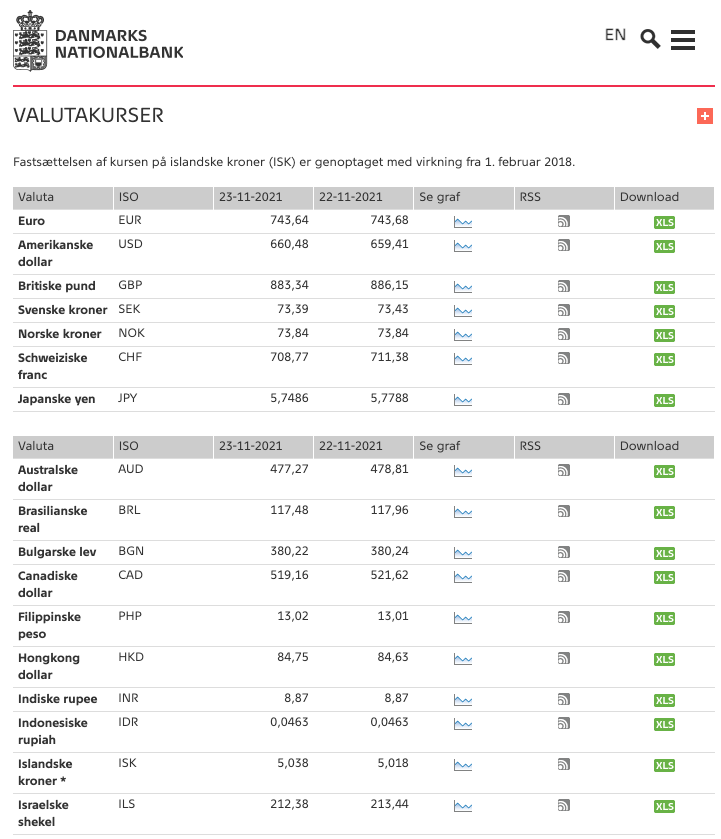
\includegraphics[width=1.2\textwidth]{valutakurser.png}
\end{minipage}

\shead{Regulært udtryk til at udtrække værdien}

\begin{lstlisting}[numbers=none,frame=none]
let floatregex = "([1-9][0-9]*,[0-9]+)"
let regex = "EUR.*\\n.*>" + floatregex + "<"
\end{lstlisting}

\end{footnotesize}
\end{frame}

\begin{frame}[fragile]
\begin{footnotesize}
  \shead{``Scraping'' af valutakurser --- Implementation (\lstinline{fetchfx.fs})}

\begin{lstlisting}[numbers=none,frame=none]
// Find FX rate for a particular currency
let findfx cur s =
  let floatregex = "([1-9][0-9]*,[0-9]+)"
  let regex = cur + ".*\\n.*>" + floatregex + "<"
  in match extract (Regex regex) s with
      | Some v -> v
      | None -> "error"

do printf "Enter currency (CUR): "
let cur = System.Console.ReadLine()
let cur_regex = Regex "USD|EUR|CHF|SEK|NOK|GBP|AUD|JPY|CAD"

if cur_regex.IsMatch cur then
  let s = fetchUrl "https://www.nationalbanken.dk/valutakurser"
  let fx = findfx cur s
  do printfn "%sDKK=%s" cur fx
else
  do printfn "Currency '%s' not supported" cur
\end{lstlisting}

\end{footnotesize}
\end{frame}

\begin{frame}[fragile]
\begin{footnotesize}
  \shead{``Scraping'' af valutakurser --- Brug af løsningen}

\begin{verbatim}
bash-3.2$ fsharpc --nologo fetchfx.fs
bash-3.2$ mono fetchfx.exe
Enter currency (CUR): USD
USDDKK=659,41
bash-3.2$ mono fetchfx.exe
Enter currency (CUR): CAD
CADDKK=521,62
bash-3.2$
\end{verbatim}

\vspace{1ex}

\shead{Bemærk:}
\begin{itemize}
\item Løsningen afhænger af at web-sitet der scrapes fra ikke ændrer format.
\item Dette eksempel er kun vist som et eksempel på hvad der er
  teknisk muligt.
\item Der kan være juridiske problemer med at ``scrape'' data fra web-sites...
\end{itemize}
\end{footnotesize}
\end{frame}

\subsection*{Konklusion}
\begin{frame}[fragile]
  \headsp{Konklusion}

  \vspace{3mm}
  \tableofcontents
\end{frame}

\end{document}
